\documentclass[letter,10pt]{article}
\usepackage[utf8]{inputenc}
\usepackage[english]{babel}
\usepackage{fancyvrb}
\usepackage{fancyhdr}
\usepackage{url}
\usepackage{verbatim}
\usepackage{graphicx}
\usepackage{rotating}
\usepackage{listings}
\usepackage{float}


\lstset{
language=C
}

\parskip 1mm
\setlength{\topmargin}{0pt}
\oddsidemargin  0.5cm
\evensidemargin 0.5cm
\textwidth      15.5cm
\textheight     21.0cm
\headsep        4 mm
\parindent      0.5cm

\pagestyle{fancyplain}

\lhead{Estadística Computacional 2015}
\rhead{\bf \it LEC 1 }
\lfoot{}
\cfoot{}
\rfoot{\bf \thepage}
\renewcommand{\footrulewidth}{0.4pt}

\title{LEC1 \\ Estadística Computacional 2015-1, UTFSM }
\author{Gonzalo Moya 201173016-k}

\date{\vspace*{1cm} Valparaíso, 15 de Noviembre del 2015}

\newpage

\begin{document}
\maketitle
\thispagestyle{empty}
\newpage
\tableofcontents

\makeatother

\newpage

\section{Introducción}

Este infrome aborda distintos problemas de probabilidad basándose en la noción frecuentista de esta con el fin de analizar
el cómo la simulación de experimentos nos permite relacionar la probabilidad empírica con la probabilidad teórica, demostrando como la
primera converge a la segunda y por tanto probando que la simulación es un método correcto para estudiar probabilidades.


\section{Desarrollo}
\subsection{Pregunta 1}
El problema en cuestión es el famoso Monty Hall Problem para un caso particular de 5 puertas.
\begin{itemize}
 \item[a)] El jugador en cuestión inicialmente tenía la probabilidad de $\frac{1}{5}$ de acertar a la puerta, una vez que el presentador
 abre una puerta y a su vez el participante decide cambiar de elección entonces las otras 3 puertas restantes tienen 
 \item[b)]
 \item[c)]
\end{itemize}

\subsection{Pregunta 2}
?
\subsection{Pregunta 3}
?
\subsection{Pregunta 4}
\begin{itemize}
 \item[a)] Para responder a la pregunta se realizan distintos experimentos para $n= 100,500,1000,1500$, A continuación se muestra el para $n=100$.
    0    1    2    3    4    5    6    7 
0.03 0.10 0.32 0.60 0.88 0.98 0.99 1.00 

 p real
[1] 0.01822838 0.10800994 0.30700341 0.56836796 0.79364860 0.92679954 0.98145105
[8] 0.99683271

suma [1] 0.2156783
  \begin{minipage}{\linewidth}
      \centering
      \begin{minipage}{0.45\linewidth}
          \begin{figure}[H]
              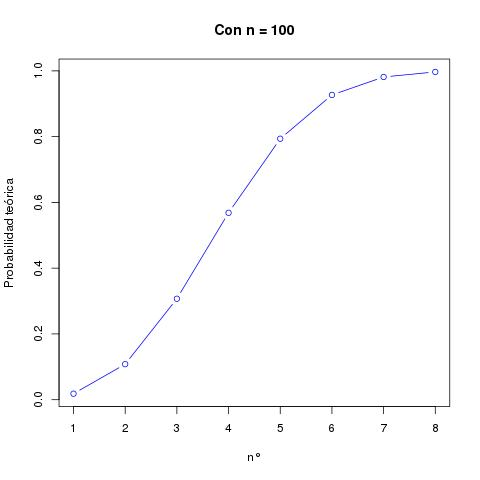
\includegraphics[width=\linewidth]{p3_teo_100.jpg}
              \caption{P. Te\'orica para n = 100}
          \end{figure}
      \end{minipage}
      \hspace{0.05\linewidth}
      \begin{minipage}{0.45\linewidth}
          \begin{figure}[H]
              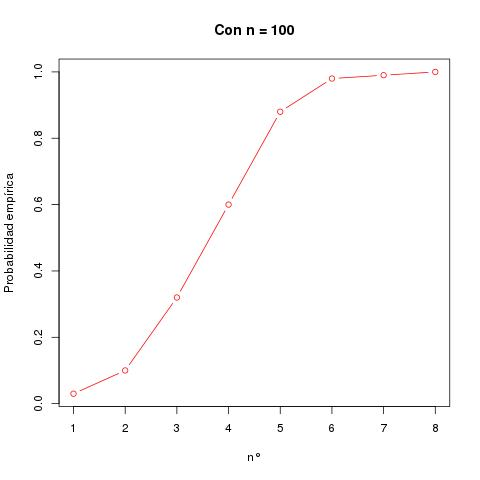
\includegraphics[width=\linewidth]{p3_emp_100.jpg}
              \caption{P. Emp\'irica para n = 100}
          \end{figure}
      \end{minipage}
  \end{minipage}


Para n = 500

frec acum
    0     1     2     3     4     5     6     7     8 
0.024 0.116 0.304 0.552 0.756 0.934 0.984 0.992 1.000


[1] 0.01822838 0.10800994 0.30700341 0.56836796 0.79364860 0.92679954 0.98145105
[8] 0.99683271 0.99967373

[1] 0.08569003


  \begin{minipage}{\linewidth}
      \centering
      \begin{minipage}{0.45\linewidth}
          \begin{figure}[H]
              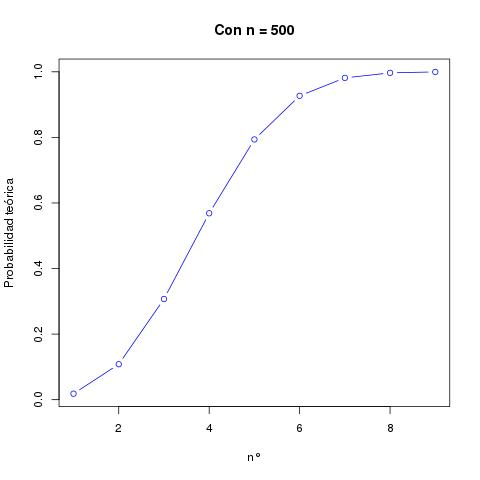
\includegraphics[width=\linewidth]{p4_teo_500.jpg}
              \caption{P. Te\'orica para n = 500}
          \end{figure}
      \end{minipage}
      \hspace{0.05\linewidth}
      \begin{minipage}{0.45\linewidth}
          \begin{figure}[H]
              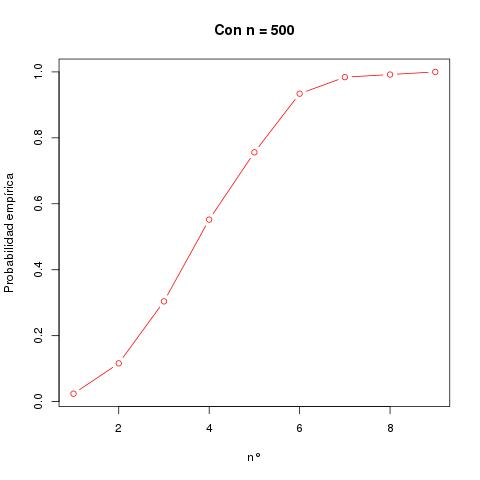
\includegraphics[width=\linewidth]{p4_emp_500.jpg}
              \caption{P. Emp\'irica para n = 500}
          \end{figure}
      \end{minipage}
  \end{minipage}
  
 frec acum
    0     1     2     3     4     5     6     7     8     9 
0.033 0.127 0.318 0.583 0.804 0.938 0.982 0.996 0.998 1.000 
 p real
 [1] 0.01822838 0.10800994 0.30700341 0.56836796 0.79364860 0.92679954 0.98145105
 [8] 0.99683271 0.99967373 0.99998468
 suma
[1] 0.08401288

  \begin{minipage}{\linewidth}
      \centering
      \begin{minipage}{0.45\linewidth}
          \begin{figure}[H]
              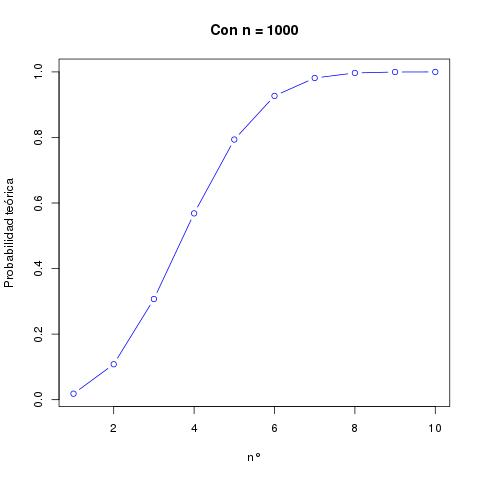
\includegraphics[width=\linewidth]{p4_teo_1000.jpg}
              \caption{P. Te\'orica para n = 1000}
          \end{figure}
      \end{minipage}
      \hspace{0.05\linewidth}
      \begin{minipage}{0.45\linewidth}
          \begin{figure}[H]
              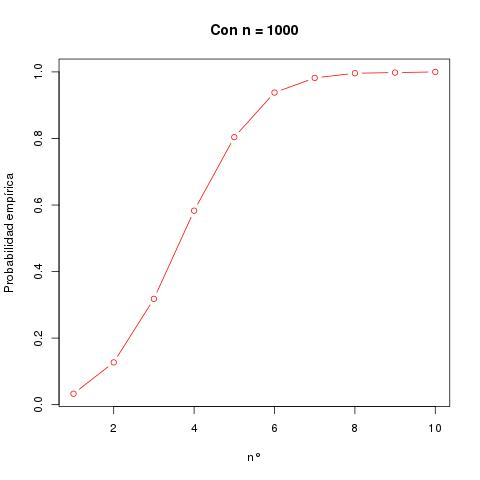
\includegraphics[width=\linewidth]{p4_emp_1000.jpg}
              \caption{P. Emp\'irica para n = 1000}
          \end{figure}
      \end{minipage}
  \end{minipage}
  
  
  
  
 frec acum
         0          1          2          3          4          5          6 
0.02133333 0.11333333 0.30800000 0.56066667 0.79533333 0.92000000 0.97800000 
         7          8 
0.99600000 1.00000000 
p real
[1] 0.01822838 0.10800994 0.30700341 0.56836796 0.79364860 0.92679954 0.98145105
[8] 0.99683271 0.99967373
suma
[1] 0.03022055
 
  \begin{minipage}{\linewidth}
      \centering
      \begin{minipage}{0.45\linewidth}
          \begin{figure}[H]
              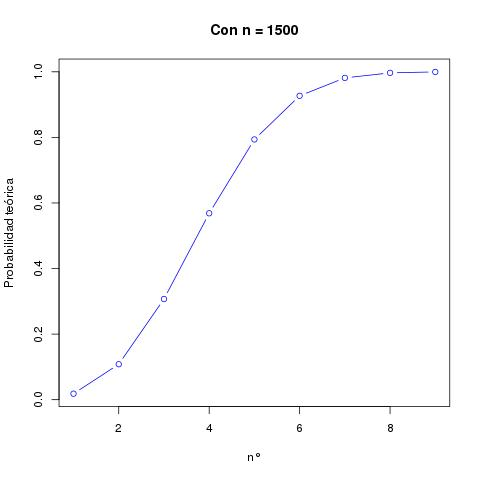
\includegraphics[width=\linewidth]{p4_teo_1500.jpg}
              \caption{P. Te\'orica para n = 1500}
          \end{figure}
      \end{minipage}
      \hspace{0.05\linewidth}
      \begin{minipage}{0.45\linewidth}
          \begin{figure}[H]
              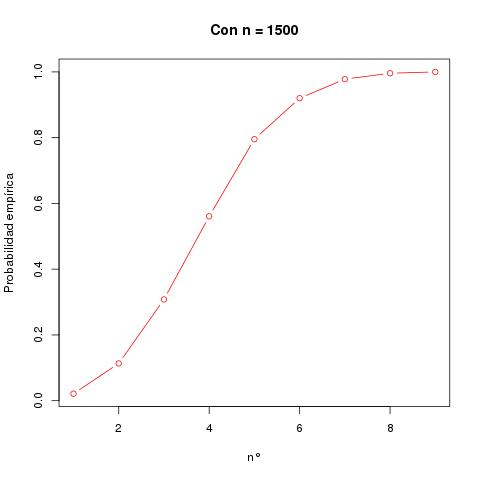
\includegraphics[width=\linewidth]{p4_emp_1500.jpg}
              \caption{P. Emp\'irica para n = 1500}
          \end{figure}
      \end{minipage}
  \end{minipage}

  
frec acum
      0       1       2       3       4       5       6       7       8       9 
0.01827 0.10744 0.30679 0.57137 0.79618 0.92856 0.98189 0.99710 0.99967 1.00000 
 p real
 [1] 0.01822838 0.10800994 0.30700341 0.56836796 0.79364860 0.92679954 0.98145105
 [8] 0.99683271 0.99967373 0.99998468
 suma
[1] 0.008844152
 
 
  \begin{minipage}{\linewidth}
      \centering
      \begin{minipage}{0.45\linewidth}
          \begin{figure}[H]
              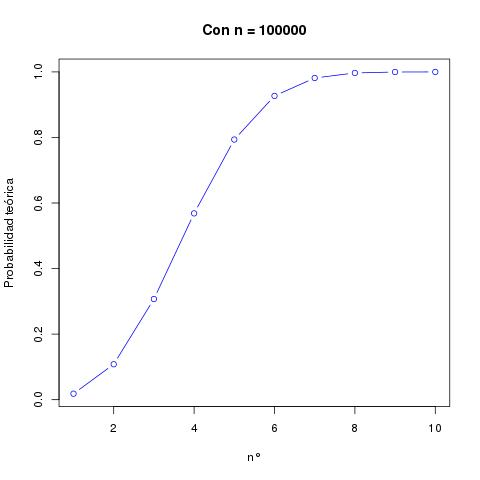
\includegraphics[width=\linewidth]{p4_teo_100000.jpg}
              \caption{P. Te\'orica para n = 100000}
          \end{figure}
      \end{minipage}
      \hspace{0.05\linewidth}
      \begin{minipage}{0.45\linewidth}
          \begin{figure}[H]
              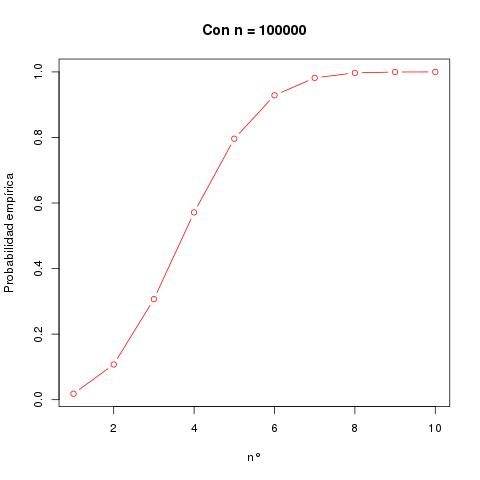
\includegraphics[width=\linewidth]{p4_emp_100000.jpg}
              \caption{P. Emp\'irica para n = 100000}
          \end{figure}
      \end{minipage}
  \end{minipage}
  
\item[b)]
Finalmente para un $n = 100000$ se encuentra una convergencia menor a 0.01, para el caso puntual
es de 0.008844152.
 
\end{itemize}

\subsection{Pregunta 5}
\subsection{Pregunta 6}
\subsection{Pregunta 7}
\subsection{Pregunta 8}




\section{Conclusiones}


%\section{Anexos}


%\bibliographystyle{alpha}
%\bibliography{bibbase}

% referencias
%[1] Nombre de la referencia, Autor.



\end{document}
